%%%%%%%%%%%%%%%%%%%%%%%%%%%%%%%%%%%%%%%%%
% Template information:
% Template name: Ernie's Article
% Version: 1.0 (2023.03.26)
% Author: 莊程翔 Ernie Cheng-Xiang Zhuang
% Complier: XeLaTeX -> BibTeX -> XeLaTeX -> XeLaTeX
%
% The purpose of making this template:
% Due to its steep learning curve, LaTeX is not particularly beginner-friendly, while Word may not be aesthetically pleasing when it comes to typesetting mathematical equations and Chinese characters. Therefore, I have created this template, complete with clear and concise comments, numerous useful packages, and customized commands to enable LaTeX beginners to easily complete assignments, reports, and even theses.
% If you have any questions, you can contact me by:
% 1. Website: https://www.ernie-zhuang.com/contact
% 2. Email: erniezhuang1127@gmail.com
%%%%%%%%%%%%%%%%%%%%%%%%%%%%%%%%%%%%%%%%%

%----------------------------------------------------------------------------------------
%	Packages and Document Configurations
%----------------------------------------------------------------------------------------

\documentclass[utf8,12pt]{article} % Set font size and UTF-8 encoding

%%%%%%%%%%%%%%%%%%%%%%%%%%%%%%%%%%%%%%%%%
% Template information:
% Template name: Ernie's Article
% Version: 1.0 (2023.03.26)
% Author: 莊程翔 Ernie Cheng-Xiang Zhuang
% Complier: XeLaTeX -> BibTeX -> XeLaTeX -> XeLaTeX
%
% The purpose of making this template:
% Due to its steep learning curve, LaTeX is not particularly beginner-friendly, while Word may not be aesthetically pleasing when it comes to typesetting mathematical equations and Chinese characters. Therefore, I have created this template, complete with clear and concise comments, numerous useful packages, and customized commands to enable LaTeX beginners to easily complete assignments, reports, and even theses.
% If you have any questions, you can contact me by:
% 1. Website: https://www.ernie-zhuang.com/contact
% 2. Email: erniezhuang1127@gmail.com
%%%%%%%%%%%%%%%%%%%%%%%%%%%%%%%%%%%%%%%%%

%----------------------------------------------------------------------------------------
%	Packages and Document Configurations
%----------------------------------------------------------------------------------------

% Output font encoding by Type 1
\usepackage[T1]{fontenc} 

% Specification of custom fonts
\usepackage{fontspec} 

%% Specified font
\setmainfont{Times New Roman} 

% Use A4 paper and set left, right, top and bottom margins
\usepackage[left=3.18cm, right=3.18cm, top=2.54cm, bottom=2.54cm]{geometry} 

% Line spacing, with \begin{spacing}{1.5} and \end{spacing}
\usepackage{setspace} 

% Blank line for the first line of text in each paragraph
\usepackage{indentfirst} 

% Set the first line of each paragraph to be empty 2 characters (2em)
\setlength{\parindent}{2em} 

% Set any font size (such as 13.5pt)
\usepackage{type1cm} 

% Sets the section numbering style (Comment out this one up to \usepackage{color} with a % if you don't want to change the section style.)
\usepackage{titletoc} % Adjust the form of section title
\usepackage[small]{titlesec} % Modify section font and size. (you can add small, sf in square brackets)
%\renewcommand\thesection{\arabic{section}} % adjustment section number (It can changed to: \Alph, \alph, \Roman, \roman)
%\renewcommand\thesubsection{\arabic{section}.\arabic{subsection}.} % adjustment subsection number
%\renewcommand\thesubsubsection{\arabic{section}.\arabic{subsection}.\alph{subsubsection}} % adjustment subsubsection number
%\makeatletter

% Required for custom colors
\usepackage{color} 

%% Color section titles
\definecolor{NTHU_Purple}{RGB}{126,35,138}
\definecolor{Default_Blue}{RGB}{52,51,171}

% Math tools and symbols
\usepackage{mathtools, amsmath, amsfonts, amsthm, latexsym} 

% Increase the space between mathematical symbols and make the ones bold
\usepackage{newtxtext,newtxmath}

\theoremstyle{definition} % The style of mathematical theorems and definitions (It can be changed to: plain, remark, definition, thmsty)
\newtheorem{Assum}{\textbf{Assumption}}
\newtheorem{Axiom}{\textbf{Axiom}}
\newtheorem{Def}{\textbf{Definition}}
\newtheorem{Thm}{\textbf{Theorem}}
\newtheorem{Lemma}{\textbf{Lemma}}
\newtheorem{Corol}{\textbf{Corollary}}
\newtheorem{Property}{\textbf{Property}}
\newtheorem{Proposition}{\textbf{Proposition}}
\newtheorem{Claim}{\textbf{Claim}}
\newtheorem{Remark}{\textbf{Remark}}
\newtheorem{Note}{\textbf{Note}}
\renewcommand{\proofname}{\textbf{proof.}}

% Correct: \Checkmark; Wrong(Cross): \XSolid
\usepackage{bbding} 

% Sets the position of figure and table titles
\usepackage[justification=centering]{caption} 
\usepackage[justification=centering, format=hang]{subcaption}

% Set the font size and series of automatic numbering
\captionsetup[figure]{font=normalsize, labelfont=md}
\captionsetup[table]{font=normalsize, labelfont=md}

% Insert graphics and tables
\usepackage{graphicx}  % \scalebox{} can be used to scale down an overly large table
\usepackage{booktabs}

% Multiple row
\usepackage{multirow} 

% Array
\usepackage{array}

% Flip table 90 degrees counterclockwise
\usepackage{lscape} 

% Long table (table across pages)
\usepackage{longtable} 

% Numbers in the table, aligned with decimal points or commas
\usepackage{dcolumn} 

% Adjust the position of the graph
\renewcommand{\textfraction}{0.15}
\renewcommand{\topfraction}{0.85}
\renewcommand{\bottomfraction}{0.85}
\renewcommand{\floatpagefraction}{0.60}

% Adjust the alignment of numbers in tables
\newcolumntype{d}[1]{D{,}{,}{#1}} % Aligned with commas, you should type d{?} when arranging the table
\newcolumntype{.}[1]{D{.}{.}{#1}} % To align with a decimal point, you should type .{?} when arranging the table

% wrap figure
\usepackage{wrapfig} 

% Increase the spacing between footnotes
\setlength{\footnotesep}{1em} 

% Colors for links
\usepackage{url}
\usepackage[colorlinks, bookmarks = false]{hyperref}

%% Set colors for links
\hypersetup{
	linkcolor = black,
	citecolor = blue,
	filecolor = blue,
	urlcolor = blue
} 

% Enumerate itrm
\usepackage{enumerate} 

% Commenting out large sections
\usepackage{comment}

% Insert PDF pages
\usepackage{pdfpages}  % \includepdf[pages=-]{file name}

% Abstract
\usepackage{abstract} 
\renewcommand{\abstractnamefont}{\Large} % Set the size of Abstract

% Appendix
\usepackage{appendix} 
\renewcommand{\appendixpagename}{\Large \textbf{Appendices}} % Set the size of Appendices

% Citing references
\usepackage[sort]{natbib}

% Formatting Manually Cited References
\newcommand\laref{\bigskip\noindent\hangindent=1em} 

% Modify the header and footer
%\usepackage{fancyhdr} 
%\pagestyle{fancy} % Set the display style of header and footer, including empty, plain, headings, myheadings, fancy.
%\renewcommand{\sectionmark}[1]{\markright{\thesection#1}} 
%\fancyhead[LO, LE]{}
%\fancyhead[RO, RE]{\rightmark}
%\addtolength{\headheight}{6pt}
%\renewcommand{\footrulewidth}{0pt}
%\extrarowheight=2pt
 % Input packages and our setting in structure.tex

%----------------------------------------------------------------------------------------
%	文章資訊
%----------------------------------------------------------------------------------------

% 名稱
\title{How to do the \LaTeX{}  Beamer?}

% 作者
\author{% 
Ernie Cheng-Xiang Zhuang one \thanks{National Tsing Hua University one} \and%
Ernie Cheng-Xiang Zhuang two \thanks{National Tsing Hua University two}
}

% Date
\date{\today}

\begin{document}

\pagenumbering{roman} % form of page number

%----------------------------------------------------------------------------------------
%	Title
%----------------------------------------------------------------------------------------
%
\maketitle 
%
%----------------------------------------------------------------------------------------
%	Abstract
%----------------------------------------------------------------------------------------
%
\begin{abstract}\fontsize{12}{20pt}
\begin{spacing}{1.5}
This paper develops a dynamic industry model with heterogeneous firms to analyze the intra-industry effects of international trade.
The model shows how the exposure to trade will induce only the more productive firms to enter the export market
(while some less productive firms continue to produce only for the domestic market)
and will simultaneously force the least productive firms to exit.
It then shows how further increases in the industry's exposure to trade lead to additional inter-firm reallocations towards more productive firms.
The paper also shows how the aggregate industry productivity growth generated by the reallocations contributes to a welfare gain,
thus highlighting a benefit from trade that has not been examined theoretically before.
The paper adapts Hopenhayn's (1992a) dynamic industry model to monopolistic competition in a general equilibrium setting.
In so doing, the paper provides an extension of Krugman's (1980) trade model that incorporates firm level productivity differences.
Firms with different productivity levels coexist in an industry because each firm faces initial uncertainty concerning its productivity before making an irreversible investment to enter the industry.
Entry into the export market is also costly, but the firm's decision to export occurs after it gains knowledge of its productivity.

\bigskip
\noindent
\textbf{Keywords}: Intra-industry trade, firm heterogeneity, firm dynamics, selection.

\bigskip
\noindent
This abstract is taken from \href{https://www.jstor.org/stable/1555536}{\citet{melitz2003}}.
\end{spacing}
\end{abstract}
%
%----------------------------------------------------------------------------------------
%	Table of Contents
%----------------------------------------------------------------------------------------
%
\newpage
\begin{spacing}{1.5}
\tableofcontents
%
% List of Figures
\newpage
\listoffigures
%
% List of Tables
\newpage
\listoftables
%
\end{spacing}
%
%----------------------------------------------------------------------------------------
%	Sentence
%----------------------------------------------------------------------------------------
%
\newpage
\pagenumbering{arabic} % form of page number
\section{Sentence}
\begin{spacing}{1.5}
%
% \textcolor{red}{} can make the words appear in red
% \textbf can make the words appear in bold
% \textit can make the words appear in italics
 \textcolor{red}{Econometrics} is a \textbf{statistical} method used to \textit{estimate} the economic relationship,
 	test economic theories, and evaluate the effects of government or business policies.

% quote
\begin{quote}
	Pure mathematics is, in its way, the poetry of logical ideas.\\
	--- Albert Einstein
\end{quote}
%
\end{spacing}
%
%----------------------------------------------------------------------------------------
%	Itemize and Enumerate
%----------------------------------------------------------------------------------------
%
\newpage
\section{Itemize and Enumerate}
\begin{spacing}{1.5}
%
\begin{itemize} % item of `itemize' package
\item This is an item of `itemize' package
		\begin{enumerate}[a] % item of 'enumerate' package with typing a in []
			\item In Beamer, you can enter nothing inside the $[]$ to generate a solid circle, but you cannot enter it in Article.
			\item This is an item of `enumerate' package with typing `a' in $[]$
			\begin{itemize} % item of `itemize' package
				\item This is an item of `itemize' package in second layer
				\begin{enumerate}[1] % item of 'enumerate' package with typing 1 in []
					\item This is an item of `enumerate' package with typing `1' in $[]$
					\item This is an item of `enumerate' package with typing `1' in $[]$
				\end{enumerate}
			\end{itemize}
		\end{enumerate}
\end{itemize}
\end{spacing}
%
%----------------------------------------------------------------------------------------
%	Math
%----------------------------------------------------------------------------------------
%
\section{Math}
%
%----------------------------------------------------------------------------------------
%
\subsection{Theorem}
%
%----------------------------------------------------------------------------------------
%
\begin{spacing}{1.5}
%
\begin{Def}
	Let $f\left(x\right)$ be a function defined on an interval that contains $x=c$,
	except that possibly at $x=c$. Then we say that,
	$\lim\limits_{x\rightarrow c} f\,(x)=L$
	if for every number $\epsilon > 0$ there is some number  $\delta > 0$ such that
	$\left\vert f(x)-L \right\vert < \epsilon$ whenever $0<\left\vert x-c \right\vert < \delta$.
\end{Def}

\begin{Axiom}
	Axioms can be specified using Axiom's environment command.
\end{Axiom}

\begin{Assum}
	Assumptions can be specified using Assum's environment command.
\end{Assum}

\begin{Thm}
	Theorems can be specified using Thm's environment command.
\end{Thm}

\begin{Lemma}
	Lemmas can be specified using Lemma's environment command.
\end{Lemma}

\begin{Corol}
	Corollaries can be specified using Corol's environment command.
\end{Corol}

\begin{Property}
	Properties can be specified using Property's environment command.
\end{Property}

\begin{Proposition}
	Propositions can be specified using Proposition's environment command.
\end{Proposition}

\begin{Claim}
	Claims can be specified using Claim's environment command.
\end{Claim}

\begin{Remark}
	Remarks can be specified using Remark's environment command.
\end{Remark}

\begin{Note}
	Notes can be specified using Note's environment command.
\end{Note}

\begin{proof}
	Proof can be specified using proof's environment command.
\end{proof}
%
\end{spacing}
%
%----------------------------------------------------------------------------------------
%
\subsection{Mathematical Equations}
%
%----------------------------------------------------------------------------------------
%
% In mathematical equations, we often use symbols to adjust spacing as needed.
%% \, plus 1.5pt 
%% \! minus 1.5pt
%% \: plus 3pt
%% \; plus 5pt
\begin{align}\label{reg}
	\ln\left[\frac{Prob.\left(Y=b|X\right)}{Prob.\left(Y=0|X\right)}\right]
		=\beta_0+\sum_{j=1}^k \beta_{i,j}\,X_{i,j,b|Y=0}+\varepsilon_{i,b|Y=0}
\end{align}
%
\begin{align}\label{var}
	\left(n-1\right)\!S^{\,2} & =  \sum_{i=1}^{n}\left(x_{i}-\widebar{X}\right)^{2} 
		 =  \sum_{i=1}^{n}x_i^{\,2}-n\widebar{X}^{\,2} \notag \\
	\Rightarrow \sum_{i=1}^{n} x_i^{\,2} & =  \left(n-1\right)\!S^{\,2}+\underbrace{n \widebar{X}^{\,2}}_{\text{校正項}}
\end{align}
%
%----------------------------------------------------------------------------------------
%	Figure and Table
%----------------------------------------------------------------------------------------
%
\section{Figure and Table}
%
%----------------------------------------------------------------------------------------
%
\subsection{Single Figure}
%
%----------------------------------------------------------------------------------------
%
\begin{figure}[htbp]
	\centering % Centering
	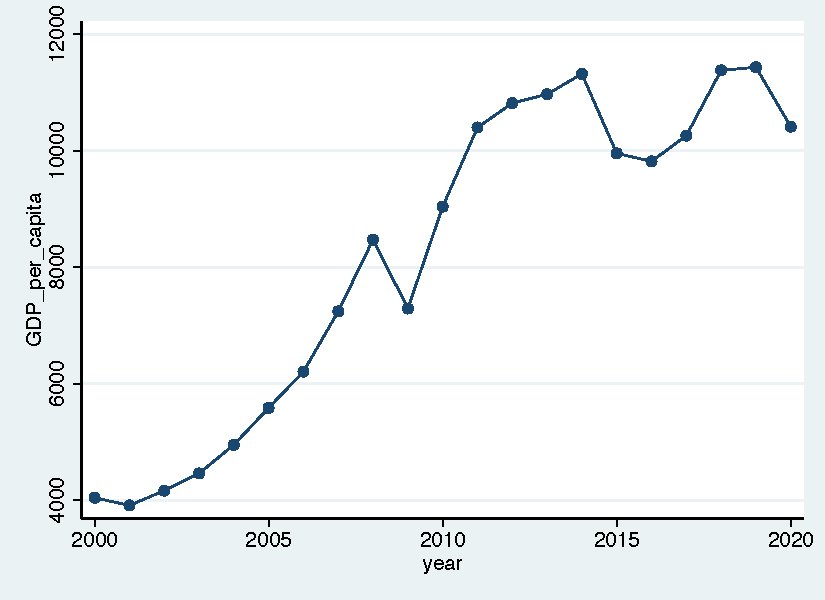
\includegraphics[scale=0.8]{Fig/GDP_per_capita.pdf}\\ % Insert a figure
	\hspace{-19em}\footnotesize{Sources: Worldbank.}\\ % Adjust position and insert sources
	\caption{GDP per capita in Malaysia (current US\$)} % Figure name
	\label{GDP_per_capita} % Figure label
\end{figure}
%
%----------------------------------------------------------------------------------------
%
\subsection{Subfigure}
%
%----------------------------------------------------------------------------------------
%
\begin{figure}[htbp]
	\centering 
	\begin{subfigure}[b]{0.45\textwidth} % Adjust column width
		\centering 
		
\includegraphics[width=\textwidth]{Fig/LaTeX}\\
		\footnotesize{Sources: 
		\href{https://en.wikipedia.org/wiki/LaTeX}{Wiki}.}
		\caption{\LaTeX~1} 
		\label{LaTeX 1} % Subfigure label
	\end{subfigure}
	\hfill
	\begin{subfigure}[b]{0.45\textwidth}
		\centering
		
\includegraphics[width=\textwidth]{Fig/LaTeX}
		\footnotesize{Sources: 
		\href{https://en.wikipedia.org/wiki/LaTeX}{Wiki}.}
		\caption{\LaTeX~2} 
		\label{LaTeX 2} % Subfigure label
	\end{subfigure}
	\par
	\begin{subfigure}[b]{0.45\textwidth} % Adjust column width
		\centering 
		
\includegraphics[width=\textwidth]{Fig/LaTeX}\\
		\footnotesize{Sources: 
		\href{https://en.wikipedia.org/wiki/LaTeX}{Wiki}.}
		\caption{\LaTeX~3} 
		\label{LaTeX 3} % Subfigure label
	\end{subfigure}
	\hfill
	\begin{subfigure}[b]{0.45\textwidth}
		\centering
		
\includegraphics[width=\textwidth]{Fig/LaTeX}
		\footnotesize{Sources: 
		\href{https://en.wikipedia.org/wiki/LaTeX}{Wiki}.}
		\caption{\LaTeX~4} 
		\label{LaTeX 4} % Subfigure label
	\end{subfigure}	
	\caption{\LaTeX} 
	\label{LaTeX} % Figure label
\end{figure}
%
%----------------------------------------------------------------------------------------
%
\subsection{wrapfigure}
%
%----------------------------------------------------------------------------------------
%
\begin{spacing}{1.5}
%
\begin{wrapfigure}{R}{0.3\textwidth} % Use R or L to control the position of the plot
\centering

\includegraphics[width=0.3\textwidth]{Fig/nthulogo}\\
\footnotesize{Sources: \href{https://www.nthu.edu.tw/files/cis/cis-1.pdf}{NTHU}.}
\caption{NTHU Logo}
\end{wrapfigure}
%
National Tsing Hua University has a long and proud history. First established as the Tsing Hua Academy at Tsing Hua Garden in Beijing in 1911,
the Academy was renamed as National Tsing Hua University in 1928 as its curricula expanded to that of a full-fledged university.
In 1956, National Tsing Hua University (NTHU) was reinstalled on its current campus in Hsinchu, Taiwan.

National Tsing Hua University (NTHU) was reinstalled on its current campus in Hsinchu, Taiwan.
Since its reinstallation, NTHU has developed from an institute focusing on Nuclear Science and Technology to that of a comprehensive research university
offering degree programs ranging from baccalaureate to doctorate in science, technology, engineering, humanities and social sciences, as well as management.
NTHU has been consistently ranked as one of the premier universities in Taiwan and is widely recognized as the best incubator for future leaders in industries as well as academics.
Such stellar records are particularly exemplified by the outstanding achievements of our alumni, including two Nobel laureates in physics Drs. Cheng- Ning Yang and Tsung-Dao Lee,
one Nobel laureate in chemistry Dr. Yuan-Tseh Lee and one Wolf Prize winner in mathematics Dr. Shiing-Shen Chern.
(This article is taken from: \href{https://www.nthu.edu.tw/about/nthuIntro/en}{NTHU}.)
%
\end{spacing}
%
%----------------------------------------------------------------------------------------
%	Table
%----------------------------------------------------------------------------------------
%
%----------------------------------------------------------------------------------------
%
\subsection{Single Table}
%
%----------------------------------------------------------------------------------------
%
\begin{table}[htbp]
	\centering 
	\caption{Statistical Differences in Student Loans Between Public and Private Universities in Taiwan (Academic Year 108)} % Table name
	\extrarowheight=2pt % Extra row height
	\label{loan} % Table label
	\scalebox{1}{ % Adjust the scale of table
	\begin{tabular}{p{6cm} p{3.5cm}<{\centering} p{3.5cm}<{\raggedleft}} % Control column width and text alignment
		\toprule
		\midrule
 		& Public universities & Private universities\\
		\midrule
		Loan amount & 3,121,271,506 & 16,098,465,719 \\
		Number of students with loans & 55,715 & 187,076 \\
		Total number of students & 439,073 & 774,099 \\
		Loan amount per capita & 56,022 & 86,053 \\
		The share of total student & 12.69\% & 24.17\% \\
		\midrule
		\bottomrule
	\end{tabular}
	}
	\par\smallskip
	\hspace{-1em}\parbox{0.9\textwidth}{\footnotesize % Control the position, font size and box width of source(s) and note(s)
	Source: \href{https://helpdreams.moe.edu.tw/hd/upload/20201211_1.pdf}{Department of Help Dreams}。\par
	Note: \parbox[t]{0.7\textwidth}{\footnotesize % remember to be slightly smaller than the \textwidth of the previous two lines
	You can write a note for the table.
	}
	}
	\end{table}
%
%----------------------------------------------------------------------------------------
%
\subsection{Landscape}
%
%----------------------------------------------------------------------------------------
%
\begin{landscape}
\begin{table}[htbp]
\centering
\caption{Logistic regression results of studying in national universities and ordinary universities}
\label{logit}
\begin{tabular}{lccccccc}
\toprule
\midrule
\multirow{3}{*}{} & \multicolumn{3}{c}{Study in a national university} & \multicolumn{3}{c}{Studying in an ordinary university} \\ 
& \multicolumn{3}{c}{(relative to studying in a private university)} & \multicolumn{3}{c}{(relative to studying in a technical university)} \\ \cmidrule(r){2-4}  \cmidrule(r){5-7} 
 & (1-1) & (1-2) & (1-3) & (2-1) & (2-2) & (2-3) \\ 
 \midrule
Parents' socio-economic status &  &  &  &  &  &  \\
\hspace{1em} \multirow{2}{*}{Dad: Low; Mom: Middle} & 0.039 & 0.041 & 0.023 & 0.545** & 0.546** & 0.528** \\
 & (0.191) & (0.191) & (0.195) & (0.174) & (0.174) & (0.179) \\
\hspace{1em} \multirow{2}{*}{Dad: Low; Mom: High} & 0.183 & 0.188 & 0.163 & 0.745*** & 0.748*** & 0.813*** \\
 & (0.200) & (0.200) & (0.205) & (0.190) & (0.190) & (0.197) \\
\hspace{1em} \multirow{2}{*}{Dad: Low; Mom: No employment} & -0.244+ & -0.239+ & -0.206 & 0.121 & 0.123 & 0.187 \\
 & (0.138) & (0.138) & (0.140) & (0.122) & (0.123) & (0.127) \\
\hspace{1em} \multirow{2}{*}{Dad: Middle; Mom: Low} & -0.259 & -0.249 & -0.213 & 0.521 & 0.525 & 0.488 \\
 & (0.443) & (0.444) & (0.446) & (0.385) & (0.386) & (0.396) \\
\hspace{1em} \multirow{2}{*}{Dad: Middle; Mom: Middle} & 0.356 & 0.356 & 0.387 & 0.864** & 0.865** & 0.846** \\
 & (0.291) & (0.292) & (0.293) & (0.310) & (0.310) & (0.312) \\
\hspace{1em} \multirow{2}{*}{Dad: Middle; Mom: High} & 0.264 & 0.261 & 0.305 & 0.547 & 0.546 & 0.636+ \\
 & (0.385) & (0.385) & (0.388) & (0.378) & (0.378) & (0.387) \\
\hspace{1em} \multirow{2}{*}{Dad: Middle; Mom: No employment} & 0.259 & 0.255 & 0.301 & 0.887* & 0.885* & 0.901* \\
 & (0.332) & (0.333) & (0.335) & (0.374) & (0.374) & (0.376) \\
\hspace{1em} \multirow{2}{*}{Dad: High; Mom: Low} & 0.346* & 0.338+ & 0.360* & 0.455** & 0.452** & 0.508** \\
 & (0.175) & (0.175) & (0.177) & (0.170) & (0.170) & (0.173) \\
\hspace{1em} \multirow{2}{*}{Dad: High; Mom: Middle} & 0.296+ & 0.295+ & 0.323+ & 1.020*** & 1.021*** & 1.029*** \\
 & (0.178) & (0.178) & (0.179) & (0.180) & (0.180) & (0.182) \\
\hspace{1em} \multirow{2}{*}{Dad: High; Mom: High} & 0.447** & 0.445** & 0.473** & 1.466*** & 1.465*** & 1.545*** \\
 & (0.144) & (0.144) & (0.146) & (0.161) & (0.161) & (0.167) \\
 \midrule
\bottomrule
\end{tabular}
\end{table}
\end{landscape}
%
%----------------------------------------------------------------------------------------
%
\subsection{Long Table}
%
%----------------------------------------------------------------------------------------
%
\begin{longtable}{@{}crrrr@{}}
\caption{The Best 5 Jobs}\label{CareerCast}\\
%\extrarowheight=2pt 
\toprule
\midrule
Rank & 2021 &  2019 & 2018 & 2017 \\ % % the first row of the table
\midrule
\endfirsthead % End the header setting of the first table
%
\multicolumn{5}{l}{Continue from the previous page}\\[2pt] % Except for the first table, they are displayed in the upper left corner to continue the previous page.
\toprule
\midrule
Rank & 2021 &  2019 & 2018 & 2017 \\ % In addition to the first table, the first row of the table is also rendered.
\midrule
\endhead % End the table header setting except the first table.
%
\midrule
\bottomrule
\multicolumn{5}{r}{continued on next page}\\[2pt] % All but the last table are presented in the lower right corner and continued on the next page.
\endfoot\\[-10pt]  % Ends table-end setting except for the last table.
\multicolumn{5}{l}{\parbox{\textwidth}{\footnotesize % The width of this command will affect the width of the table!
Sources: \href{https://helpdreams.moe.edu.tw/hd/upload/20201211_1.pdf}{Department of Help Dreams}.\par\smallskip
Notes: \parbox[t]{0.95\textwidth}{\footnotesize % remember to be slightly smaller than the \textwidth of the previous two lines
1. In 2020, CareerCast did not announce the best jobs of the year.\\
2. STEM-related occupations in bold.
}
}
}
\endlastfoot
1 & {Data Analyst} & \textbf{Data Analyst}  &  Genetic Counselors & \textbf{Statistician} \\
2 & Genetic Counselors & \textbf{Statistician} & \textbf{Mathematician}  & M. S. Manager \\
3 & \textbf{Statistician} & University Professor  & University Professor & \textbf{OR Analyst}\\
4 &M. S. Manager & Occupational Therapy  & Occupational Therapy & \textbf{I. S. Analyst} \\
5 & \textbf{Mathematician} & Genetic Counselors & \textbf{Statistician} & \textbf{Data Analyst} \\
1 & {Data Analyst} & \textbf{Data Analyst}  &  Genetic Counselors & \textbf{Statistician} \\
2 & Genetic Counselors & \textbf{Statistician} & \textbf{Mathematician}  & M. S. Manager \\
3 & \textbf{Statistician} & University Professor  & University Professor & \textbf{OR Analyst}\\
4 &M. S. Manager & Occupational Therapy  & Occupational Therapy & \textbf{I. S. Analyst} \\
5 & \textbf{Mathematician} & Genetic Counselors & \textbf{Statistician} & \textbf{Data Analyst} \\
1 & {Data Analyst} & \textbf{Data Analyst}  &  Genetic Counselors & \textbf{Statistician} \\
2 & Genetic Counselors & \textbf{Statistician} & \textbf{Mathematician}  & M. S. Manager \\
3 & \textbf{Statistician} & University Professor  & University Professor & \textbf{OR Analyst}\\
4 &M. S. Manager & Occupational Therapy  & Occupational Therapy & \textbf{I. S. Analyst} \\
5 & \textbf{Mathematician} & Genetic Counselors & \textbf{Statistician} & \textbf{Data Analyst} \\
1 & {Data Analyst} & \textbf{Data Analyst}  &  Genetic Counselors & \textbf{Statistician} \\
2 & Genetic Counselors & \textbf{Statistician} & \textbf{Mathematician}  & M. S. Manager \\
3 & \textbf{Statistician} & University Professor  & University Professor & \textbf{OR Analyst}\\
4 &M. S. Manager & Occupational Therapy  & Occupational Therapy & \textbf{I. S. Analyst} \\
5 & \textbf{Mathematician} & Genetic Counselors & \textbf{Statistician} & \textbf{Data Analyst} \\
1 & {Data Analyst} & \textbf{Data Analyst}  &  Genetic Counselors & \textbf{Statistician} \\
2 & Genetic Counselors & \textbf{Statistician} & \textbf{Mathematician}  & M. S. Manager \\
3 & \textbf{Statistician} & University Professor  & University Professor & \textbf{OR Analyst}\\
4 &M. S. Manager & Occupational Therapy  & Occupational Therapy & \textbf{I. S. Analyst} \\
5 & \textbf{Mathematician} & Genetic Counselors & \textbf{Statistician} & \textbf{Data Analyst} \\
1 & {Data Analyst} & \textbf{Data Analyst}  &  Genetic Counselors & \textbf{Statistician} \\
2 & Genetic Counselors & \textbf{Statistician} & \textbf{Mathematician}  & M. S. Manager \\
3 & \textbf{Statistician} & University Professor  & University Professor & \textbf{OR Analyst}\\
4 &M. S. Manager & Occupational Therapy  & Occupational Therapy & \textbf{I. S. Analyst} \\
5 & \textbf{Mathematician} & Genetic Counselors & \textbf{Statistician} & \textbf{Data Analyst} \\
1 & {Data Analyst} & \textbf{Data Analyst}  &  Genetic Counselors & \textbf{Statistician} \\
2 & Genetic Counselors & \textbf{Statistician} & \textbf{Mathematician}  & M. S. Manager \\
3 & \textbf{Statistician} & University Professor  & University Professor & \textbf{OR Analyst}\\
4 &M. S. Manager & Occupational Therapy  & Occupational Therapy & \textbf{I. S. Analyst} \\
5 & \textbf{Mathematician} & Genetic Counselors & \textbf{Statistician} & \textbf{Data Analyst} \\
1 & {Data Analyst} & \textbf{Data Analyst}  &  Genetic Counselors & \textbf{Statistician} \\
2 & Genetic Counselors & \textbf{Statistician} & \textbf{Mathematician}  & M. S. Manager \\
3 & \textbf{Statistician} & University Professor  & University Professor & \textbf{OR Analyst}\\
4 &M. S. Manager & Occupational Therapy  & Occupational Therapy & \textbf{I. S. Analyst} \\
5 & \textbf{Mathematician} & Genetic Counselors & \textbf{Statistician} & \textbf{Data Analyst} \\
1 & {Data Analyst} & \textbf{Data Analyst}  &  Genetic Counselors & \textbf{Statistician} \\
2 & Genetic Counselors & \textbf{Statistician} & \textbf{Mathematician}  & M. S. Manager \\
3 & \textbf{Statistician} & University Professor  & University Professor & \textbf{OR Analyst}\\
4 &M. S. Manager & Occupational Therapy  & Occupational Therapy & \textbf{I. S. Analyst} \\
5 & \textbf{Mathematician} & Genetic Counselors & \textbf{Statistician} & \textbf{Data Analyst} \\
1 & {Data Analyst} & \textbf{Data Analyst}  &  Genetic Counselors & \textbf{Statistician} \\
2 & Genetic Counselors & \textbf{Statistician} & \textbf{Mathematician}  & M. S. Manager \\
3 & \textbf{Statistician} & University Professor  & University Professor & \textbf{OR Analyst}\\
4 &M. S. Manager & Occupational Therapy  & Occupational Therapy & \textbf{I. S. Analyst} \\
5 & \textbf{Mathematician} & Genetic Counselors & \textbf{Statistician} & \textbf{Data Analyst} \\
1 & {Data Analyst} & \textbf{Data Analyst}  &  Genetic Counselors & \textbf{Statistician} \\
2 & Genetic Counselors & \textbf{Statistician} & \textbf{Mathematician}  & M. S. Manager \\
3 & \textbf{Statistician} & University Professor  & University Professor & \textbf{OR Analyst}\\
4 &M. S. Manager & Occupational Therapy  & Occupational Therapy & \textbf{I. S. Analyst} \\
5 & \textbf{Mathematician} & Genetic Counselors & \textbf{Statistician} & \textbf{Data Analyst} \\
1 & {Data Analyst} & \textbf{Data Analyst}  &  Genetic Counselors & \textbf{Statistician} \\
2 & Genetic Counselors & \textbf{Statistician} & \textbf{Mathematician}  & M. S. Manager \\
3 & \textbf{Statistician} & University Professor  & University Professor & \textbf{OR Analyst}\\
4 &M. S. Manager & Occupational Therapy  & Occupational Therapy & \textbf{I. S. Analyst} \\
5 & \textbf{Mathematician} & Genetic Counselors & \textbf{Statistician} & \textbf{Data Analyst} \\
1 & {Data Analyst} & \textbf{Data Analyst}  &  Genetic Counselors & \textbf{Statistician} \\
2 & Genetic Counselors & \textbf{Statistician} & \textbf{Mathematician}  & M. S. Manager \\
3 & \textbf{Statistician} & University Professor  & University Professor & \textbf{OR Analyst}\\
4 &M. S. Manager & Occupational Therapy  & Occupational Therapy & \textbf{I. S. Analyst} \\
5 & \textbf{Mathematician} & Genetic Counselors & \textbf{Statistician} & \textbf{Data Analyst} \\
1 & {Data Analyst} & \textbf{Data Analyst}  &  Genetic Counselors & \textbf{Statistician} \\
2 & Genetic Counselors & \textbf{Statistician} & \textbf{Mathematician}  & M. S. Manager \\
3 & \textbf{Statistician} & University Professor  & University Professor & \textbf{OR Analyst}\\
4 &M. S. Manager & Occupational Therapy  & Occupational Therapy & \textbf{I. S. Analyst} \\
5 & \textbf{Mathematician} & Genetic Counselors & \textbf{Statistician} & \textbf{Data Analyst} \\
1 & {Data Analyst} & \textbf{Data Analyst}  &  Genetic Counselors & \textbf{Statistician} \\
2 & Genetic Counselors & \textbf{Statistician} & \textbf{Mathematician}  & M. S. Manager \\
3 & \textbf{Statistician} & University Professor  & University Professor & \textbf{OR Analyst}\\
4 &M. S. Manager & Occupational Therapy  & Occupational Therapy & \textbf{I. S. Analyst} \\
5 & \textbf{Mathematician} & Genetic Counselors & \textbf{Statistician} & \textbf{Data Analyst} \\
\midrule
\bottomrule
\end{longtable}
%
%----------------------------------------------------------------------------------------
%	引注
%----------------------------------------------------------------------------------------
%
\section{Citation}
%
%----------------------------------------------------------------------------------------
%
\begin{spacing}{1.5}
%
\begin{itemize}
	\item When we refer to previous figures, tables or equations in the text, we should cite them like this:
	\begin{itemize}
		\item  ``figure $\backslash$ref\{label\}'',
			then it will appear figure \ref{GDP_per_capita} and figure \ref{LaTeX}。
		\item  ``figure $\backslash$ref\{label\}'',
			then it will appear figure \ref{LaTeX 1}, figure \ref{LaTeX 2}, figure \ref{LaTeX 3} and figure \ref{LaTeX 4}.
		\item ``table $\backslash$ref\{label\}'',
			then it will appear table \ref{loan}, table \ref{logit} and table \ref{CareerCast}.
		\item ``equation ($\backslash$ref\{label\})'',
			then it will appear equation (\ref{reg}) and equation (\ref{var}).
	\end{itemize}
	\item Also, how to cite references:
	\begin{itemize}
		\item textual citations: \textbackslash citet\{label\}.
		\begin{itemize}
			\item For instance: \citet{melitz2003}.
		\end{itemize}	
		\item parenthetical citations: \textbackslash citep\{label\}.
		\begin{itemize}
			\item For instance: \citep{melitz2003}.
		\end{itemize}
		\item Note that the benefit of using bibtex is that it will only help you enter the references you use into the references.
			(For example, there is an article by sin1996 in ref.bib that is not cited)
		\item In addition, remind to use the bib file, the order of executing the compiler is XeLaTeX $\rightarrow$ BibTeX $\rightarrow$ XeLaTeX $\rightarrow$ XeLaTeX
			(execute several times to ensure that the results are fully presented.)
	\end{itemize}	
\end{itemize}

The advantage of citation is that when the slides are changed, there is no need to manually adjust the numbering all the time.
%
\end{spacing}
%
%----------------------------------------------------------------------------------------
%	References
%----------------------------------------------------------------------------------------
%
%\newpage
%\fancyhead[RO, RE]{References}
\addcontentsline{toc}{section}{\textbf{References}}
\bibliographystyle{apalike}
\bibliography{ref}
%
\laref \textcolor{red}{The following are entered manually.}\par
\laref Sin, C. Y. and White, H. (1996). Information criteria for selecting possibly misspecified parametric models. Journal of Econometrics, 71(1-2):207–225.
%
%----------------------------------------------------------------------------------------
%	附錄
%----------------------------------------------------------------------------------------
%
%\newpage
%\fancyhead[RO, RE]{Appendices}
\addcontentsline{toc}{section}{\textbf{Appendices}}
\appendix
\appendixpage
\section{The first section of the appendix}
%
\begin{spacing}{1.5}
%
	Provide you with more detailed figures or tables.
%
\end{spacing}
%
\section{The second section of the appendix}
%
\begin{spacing}{1.5}
%
	You can also provide your more detailed mathematical proof.
%
\end{spacing}
%
\end{document}
